\documentclass[aspectratio=169,hyperref={unicode}]{beamer}

\usetheme{Szeged}
\usecolortheme{beaver}
\usepackage{fontspec}
\usepackage{xcolor}
\usepackage{ulem}
\usepackage{hyperref}
\usepackage[german]{babel}
\usepackage{amssymb} 
\usepackage{tikz} 
\usetikzlibrary{positioning}

\tikzset{set/.style={draw,circle,inner sep=0pt,align=center}}



\title{Info on Generative AI Use}
\author{Rofaïda Rabehi \& Erik Zeiner}
\institute{Fachschaft General \& Computational Linguistics\\ \textbf{University of Tübingen}}
\date{WS 2024/25 \\ Pre-course}

\begin{document}


\frame{\titlepage}

\begin{frame}
\begin{minipage}{.5\textwidth}
	\textbf{People 'not in the know' like to mix up and misuse:}
  \begin{itemize}
  	\item Artificial Intelligence
  	 \begin{itemize}
  		\item Generative AI
  	\end{itemize}
  	\item Deep learning
  	\item Machine learning
  	\item Large Language Models
  	\item Neural Networks
  	\item ...
  \end{itemize}
\end{minipage}% 
\begin{minipage}{.5\textwidth}
  	\begin{tikzpicture}
\node[set,fill=green!20,text width=7.4cm,label={[below=180pt of rea,text opacity=1]Artificial intelligence}] 
  (ai) at (0,-0.4)  (rea) {};
\node[set,fill=blue!20,text width=5cm,label={[below=114pt of rea,text opacity=1]Machine learning}] 
  (nat) at (0,-0.4)  (rea) {};
\node[set,fill=red!20,text width=3.5cm,label={[below=66pt of int]Deep learning}] 
  (int) at (0,-0.2)  {};
\node[set,fill=olive!20,text width=1.5cm] (nat) at (0,0) {LLMs};
\end{tikzpicture}
\end{minipage}
	
\end{frame}

\begin{frame}{How can machines (and LLMs) learn?}
\begin{center}
	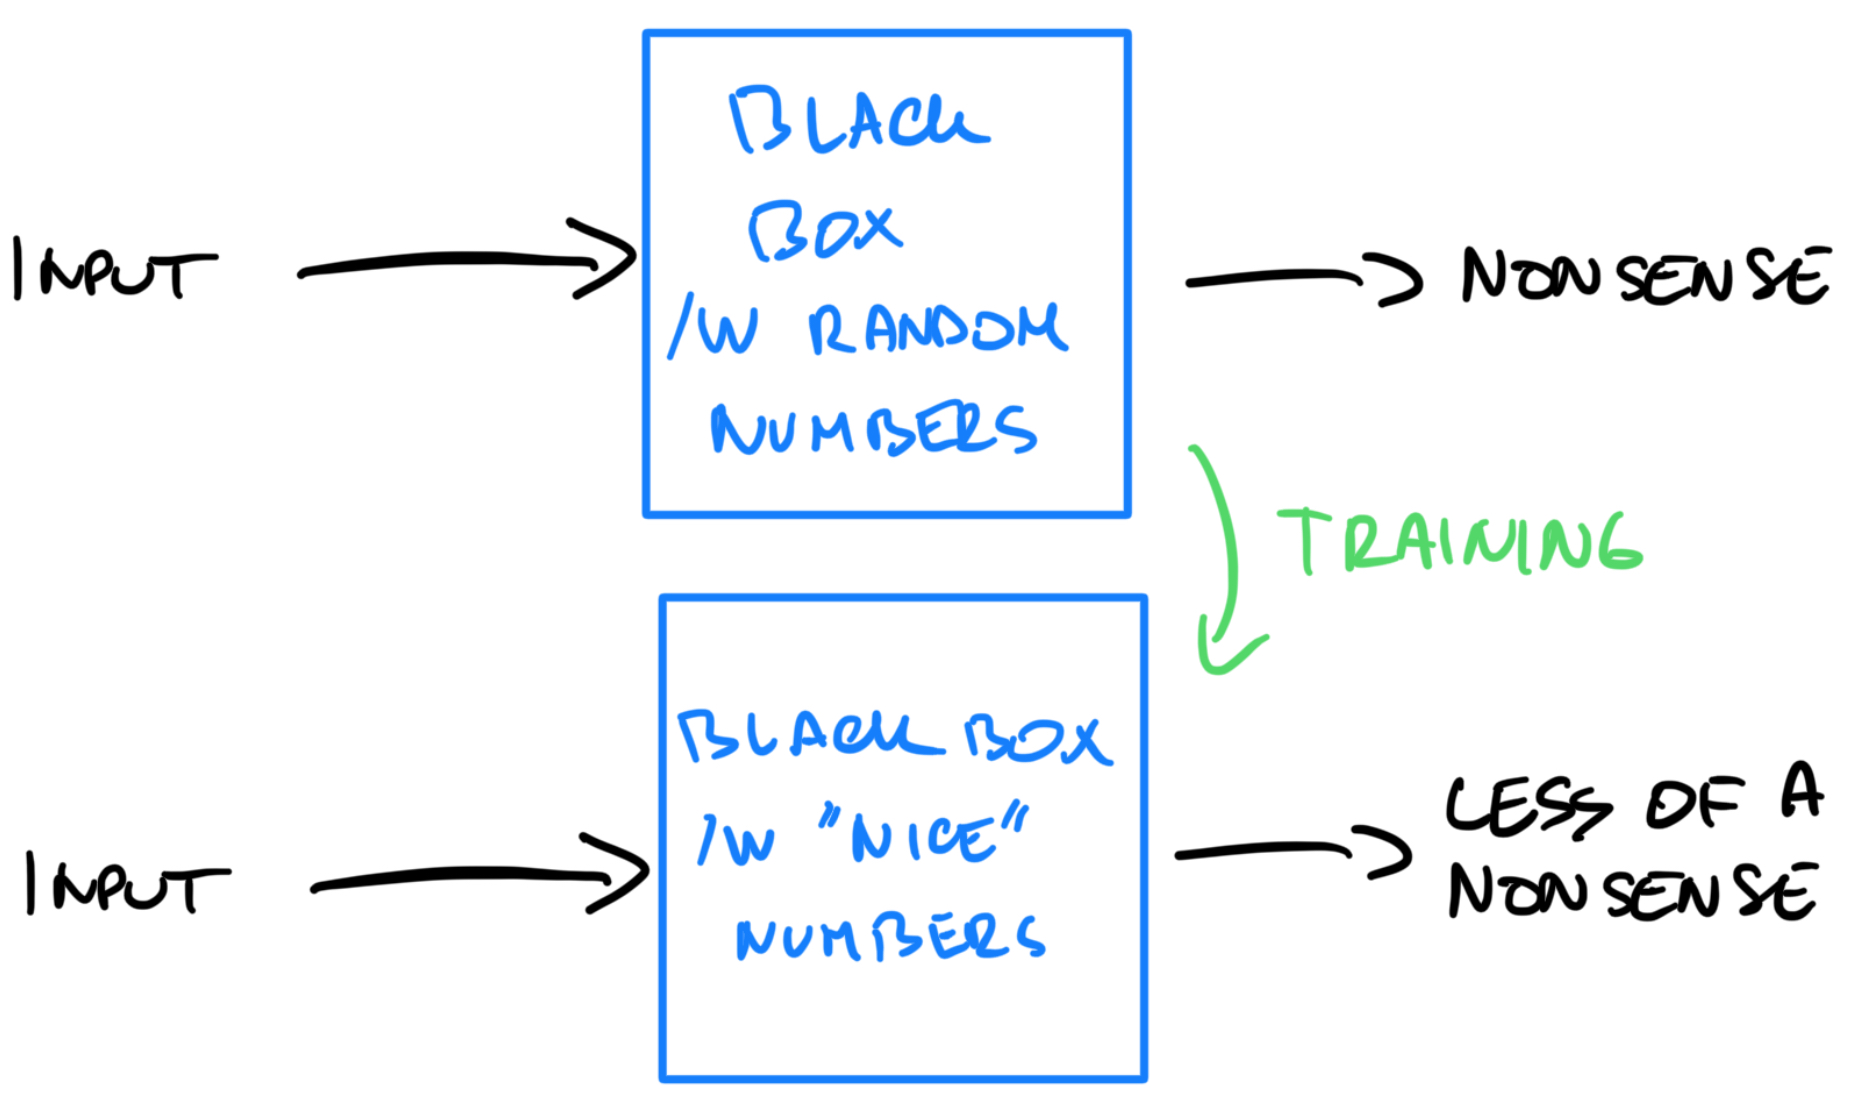
\includegraphics[scale=0.3]{training.jpg}
\end{center}
\end{frame}

\begin{frame}{Large Language Models - ChatGPT, Gemini, Claude, Llama,...}
\begin{alertblock}{Why are they models?}
attempt to 'do language' like 'we would'
\end{alertblock}

\begin{alertblock}{Why language specifically?}
trained on natural language, good for tasks such as modelling, translation, summarisation, classification,...
\end{alertblock}

\begin{alertblock}{What makes them large?}
learned knowledge about language and the world from vast amounts of text
\end{alertblock}

\end{frame}

\begin{frame}{Inherent limitations}
\begin{alertblock}{Bias}
if its in the training data, it may appear in the output\\
(toxic language, gender bias, race bias,...)
\end{alertblock}

\begin{alertblock}{Hallucinations}
prone to make things up - text is coherent, but false	
\end{alertblock}

\begin{alertblock}{Copyright/Privacy Issues}
Where did its knowledge come from?

Where did my knowledge come from?
	
\end{alertblock}

\end{frame}

\begin{frame}{Issues you might encounter}
	\begin{itemize}
		\item Doesn't actually follow the instructions or makes its own instructions to follow
		\item Gives you absolute bullshit\footnote{Hicks, M.T., Humphries, J. \& Slater, J. Correction: ChatGPT is bullshit. Ethics Inf Technol 26, 46 (2024). \url{https://doi.org/10.1007/s10676-024-09785-3}} at times
		\item You are not as sneaky as you think you are
		\item And of course, \textbf{if you outsource the learning process to someone/something else, you don't learn}
	\end{itemize}
	\end{frame}
	

\begin{frame}{Stance of the University}
	
\begin{alertblock}{The university strictly limits the usage of AI}
	As of the 31th January 2023, the University of Tübingen prohibits the usage of AI in any way, shape or form in a scientific background. Continuing the usage of any AI will lead to failing the class/module or being expelled from the university \\
 In easier words: You cant use Chatgpt not for your assignments, papers, presentations and obviously not in exams. Youll get kicked out if you do that.\\
\end{alertblock}
\end{frame}

\begin{frame}{Recommendations}
	
\begin{alertblock}{The University is aware that Generative AI is a useful tool}

 \url{https://uni-tuebingen.de/en/research/support/good-scientific-practice/guidelines-on-generative-ai/\#c2039244}

\end{alertblock}
\end{frame}


\begin{frame}{What is it good for (non-university usage)}


\begin{itemize}
\item Plugins to learn languages\\
\item Using Plug Ins \\
\item Searching for specific products\\
\item Help with installing things to your machine\\
\item Movie recommendations
\item Mundane tasks where you can verify the results
\end{itemize}

\end{frame}




\begin{frame}
\begin{center}

\textbf{Think critically, like a (computational) linguist}

---

\textbf{Don't be reliant}

---

\textbf{Use with care and consideration}


\vspace{1em}

\begin{minipage}{0.4\textwidth}
\centering
    
\includegraphics[width=0.5\textwidth]{QRtemplate_5.png}
  \end{minipage}
  \hfill
  \begin{minipage}{0.4\textwidth}
  \centering
    
\includegraphics[width=0.5\textwidth]{QRtemplate_4.png}
  \end{minipage}
\end{center}
\end{frame}
\end{document}